\documentclass[letterpaper,sansserif,tightsqueeze]{rpg-module}

\usepackage{parskip}                                                            % Add spacing between paras instead of indents
\usepackage[font=bf]{caption}
\usepackage{hyperref}
\title{Excavated Thaumaturgy}

% Compress title spacing compared to default

\addtolength{\topmargin}{-0.3cm}
\addtolength{\textheight}{0.7cm}

\begin{document}

\twocolumn

\title{Excavated Thaumaturgy}

\subtitle{Optional Rules and Miscellaneous Artifacts}

\coverimage{weapons.png}

\abstract{A compilation of OSR brain-farts and inspiring rules found on the net.}


\maketitle

\hyphenchar\font=-1
\renewcommand{\arraystretch}{1.4}

\vspace{0.5cm}
\part*{Optional Rules for Combat}
\vspace{0.5cm}

\begin{center}
	
\includegraphics[width = 0.3\linewidth]{dead.png}
\end{center}
\section{Bleeding out}
\textit{This rule is intended to add an unpredictable element to dying in battle.}

Instead of dying immediately when a damaging effect causes your HP to go to 0 or lower, you start bleeding out:
\begin{itemize}
	\item You immediately gain a pool of \textit{bleed out points}, this pool starts at 0.
	\item You have to stay prone and cannot act except for moving 5 feet.
	\item The GM rolls a d6 whenever you would normally act and increases your bleed out points by the rolled result without disclosing the either the roll or the total.
	\item The GM rolls another d6 and adds the result to the PC's total any time the PC is hit by a damaging effect.
	\item When the total is equal to or exceeds the PC's Constution score, the PC has bled out and dies.
\end{itemize}
\textbf{Applying pressure:} Other players can stop the bleeding by spending their turn taking care of the bleeding PC, the PC then becomes \textit{Stabilized}, this state is negated when the PC takes damage.

\textbf{Healing:} A downed PC can only be healed - magically or non-magically - when he or she has been stabilized. The bleed out pool is reset once the PC is healed, the bleed out score does not affect the amount of HP restored.\\

\vspace{0.5cm}

\begin{center}
	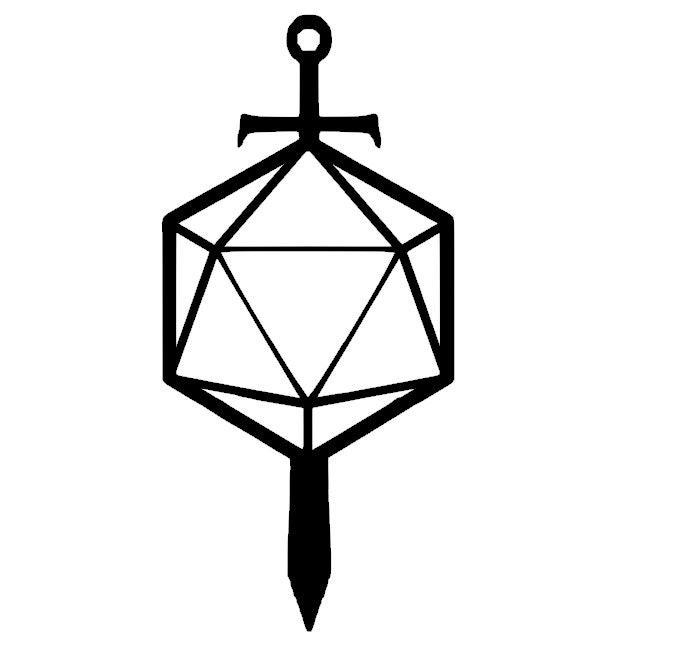
\includegraphics[width = 0.3\linewidth]{d20_weapons.jpg}
\end{center}
\section{Single D20 Combat}
\textit{Copied from a \href{https://www.youtube.com/watch?v=VflmXb0EAbI}{Bandit's Keep} video. A system that combines the attack and damage roll.}

This combat system is designed to be used in place of the standard system form B/X D\&D
The base mechanic is as follows:

\textbf{1. Ascending armor class (AAC) is used in this system.}\\
Armor worn, Dexterity and Weapon(s) increase AC\\
\textbf{2. When making an attack, the player rolls 1d20}\\
Weapon type and ability scores modify this total\\
\textbf{3. Compare the attack roll to the opponents AC}\\
If the attack roll is equal to or greater than the opponent's AC a hit is scored\\
\textbf{4. Damage equals the attack roll minus the defenders AC}\\
If the attack roll and AC are equal, a critical hit occurs

\vspace{0.5cm}

\subsection*{Rules Changes}
MAGIC-USERS can wield the following weapons:\\
Dagger, Staff, Sling

The weapon defense factor is based on weapon length and how the weapon is typically used in combat (to the best if my knowledge) thus longer weapons tend to give the greatest defense.

Daggers represent blades around 12-18 inches in length.\\
Short swords represent blades of about 24” ie Roman Gladius.\\
Swords represent blades of about 30” ie Arming Swords.\\
Two-Handed Swords have blades of about 35” ie Long Swords.\\
The much larger Great Sword would be considered a Pole Arm.

\vspace{0.5cm}

\subsection*{Calculating Armor Class}
Three factors affect Player Character (PC) Armor Class (AC)

Armor Worn (see Table \ref{table:BaseArmorClassValue} for base AC value)\\
Dexterity Score (See Table \ref{table:Dexterity})\\
Weapon Defense Bonus (See Table \ref{table:WeaponAttackAndDefenseRatings}))\\
Weapon defense ONLY affects AC against Melee attacks

Note: Monsters calculate their AC in a different manner, see section \hyperref[subsection:MonsterAC]{Calculating Monster AC}.

\begin{table}[h!]
	\centering
	\begin{tabular}{|l|l|l|}
		\hline
		\textbf{Armor Type}    & \textbf{Base Armor Class} & \textbf{Cost (in gp)} \\ \hline
		Unarmored     & 10               &              \\ \hline
		Leather Armor & 12               & 50           \\ \hline
		Chain Armor   & 14               & 150          \\ \hline
		Plate Armor   & 216              & 450          \\ \hline
		Shield        & See below        & 50           \\ \hline
	\end{tabular}
	\caption{Base Armor Class Value.}
	\label{table:BaseArmorClassValue}
\end{table}

A Shield grants an AC bonus of +3 vs melee and +5 vs missile

\begin{table}[h!]
	\centering
	\begin{tabular}{|l|l|l|}
		\hline
		\textbf{Score}	& \textbf{Missile Adjustment}	& \textbf{Armor Class Adjustment} 	\\ \hline
		3		& -3 on "to hit" rolls	& -3 Penalty				\\ \hline
		3		& -2 on "to hit" rolls	& -2 Penalty				\\ \hline
		3		& -1 on "to hit" rolls	& -1 Penalty				\\ \hline
		3		& No adjustment			& No adjustment				\\ \hline
		3		& +1 on "to hit" rolls	& +1 Bonus					\\ \hline
		3		& +2 on "to hit" rolls	& +2 Bonus					\\ \hline
		3		& +3 on "to hit" rolls	& +3 Bonus					\\ \hline
	\end{tabular}
	\caption{Dexterity.}
	\label{table:Dexterity}
\end{table}

\subsection*{Weapon Defence Bonus}
Each weapon will grant its wielder a bonus to attack and often a bonus to their AC as well, See Table B2 for details.

\subsection*{Fighting with Two Weapons}
Some weapons can be used in the off-hand (defensively) AC bonus for this use is listed in parentheses on table B2.
Example:
A thief fighting with a short sword (+4) and defending with their dagger (+1) would get a total weapon bonus of +5 to their AC

\subsection*{Missile Weapons}
Missile weapons grant no bonus to AC

\vspace{0.5cm}

\subsection*{Calculating Attack Bonus}
Three factors modify PC’s Total Attack Bonus (TAB):
\begin{itemize}
	\item PC Fighting Skill (See Table \ref{table:PCFightingSkill})
	\item Strength (Melee) or Dexterity (Missile) Score
	\item Weapon Attack Bonus (See Table \ref{table:WeaponAttackAndDefenseRatings})
\end{itemize}
Note: Monsters calculate their attack bonus in a different manner, see Section \hyperref[subsection:MonsterAC]{Calculating Monster AC}.

\begin{table}[h!]
	\centering
	\begin{tabular}{|c|c|c|c|}
		\hline
		\textbf{Fighter*}	& \textbf{Thief / Cleric}	& \textbf{Magic User}	& \textbf{Bonus}	\\
		\textbf{Level}		& \textbf{Level}			& \textbf{Level}	& \\ \hline
		1-3		& 1-4	& 1-5	& +1 	\\ \hline
		4-6		& 5-8	& 6-10	& +3  	\\ \hline
		7-9		& 9-12	& 11-14	& +6  	\\ \hline
		10-12	& 13-14	& 		& +8  	\\ \hline
		13-15	& 		& 		& +10 	\\ \hline
	\end{tabular}
	\caption{PC Fighting Skill**.}
	\label{table:PCFightingSkill}
\end{table}
\vspace{-0.5cm}
* Includes elves, dwarves and halflings.\\
** 0 level humans receive no bonus, leveled NPCs use this chart.

\begin{table}[h!]
	\centering
	\begin{tabular}{|c|c|c|c|}
		\hline
		\textbf{Weapon}	& \textbf{Attack}	& \textbf{Defense}	& \textbf{Cost (gp)}	\\
		\textbf{} 		& \textbf{Bonus}	& \textbf{Bonus}		& \textbf{}				\\ \hline
		Battle Axe*				& +6		& +1**		& 7 	\\ \hline
		Club					& +3		& 0			& 3  	\\ \hline
		Crossbow*				& Special	& Special	& 30  	\\ \hline
		Dagger/Silver			& +3		& 0 (+1)	& 3/30  \\
		Dagger					& 			& 			&		\\ \hline
		Hand Axe				& +4		& 0 (+1)	& 4 	\\ \hline
		Javelin					& Special	& Special	& 1 	\\ \hline
		Lance					& +4		& +1		& 5 	\\ \hline
		Long Bow				& Special	& Special	& 40 	\\ \hline
		Mace					& +4		& +2		& 5 	\\ \hline
		Pole Arm*				& +6		& +4		& 7 	\\ \hline
		Short Bow				& Special	& Special	& 25 	\\ \hline
		Short Sword				& +4		& +4		& 7 	\\ \hline
		Sling					& Special	& Special	& 2 	\\ \hline
		Spear					& +4		& +6		& 4 	\\ \hline
		Staff*					& +3		& +5		& 2 	\\ \hline
		Sword					& +5		& +5		& 10 	\\ \hline
		Two-Handed				& +6		& +6		& 15 	\\
		Sword*					& 			& 			&  		\\ \hline
		Warhammer				& +4		& +2		& 5 	\\ \hline
	\end{tabular}
	\caption{Weapon Attack and Defense Ratings.}
	\label{table:WeaponAttackAndDefenseRatings}
\end{table}
\vspace{-0.5cm}
* Two-handed weapon.\\
** Also destroys opponents shield on a roll that beats AC by 4 or more.

\vspace{0.5cm}

\subsection*{Missile Weapons}
Missile weapons grant no bonus to AC and add a bonus to attack rolls based on range as follows:

\begin{table}[h!]
	\centering
	\begin{tabular}{|c|c|}
		\hline
		\textbf{Range}	& \textbf{Attack Bonus}	\\ \hline
		Short	& +5 	\\ \hline
		Medium	& +4 	\\ \hline
		Large	& +3 	\\ \hline
	\end{tabular}
	\caption{Missile Attack Modifiers}
	\label{table:MissileAttackModifiers}
\end{table}

\vspace{0.5cm}

\subsection*{Other Considerations}
\textbf{Unarmed and Unarmored}\\
A PC (or human type) may add their level (or HD) to their base AC if they are unarmed AND unarmored.\\
Example:\\
Our 3rd level thief has been throw in a cell for picking pockets after being stripped to just their normal clothes. Their AC is currently 13 plus any DEX bonus.

\vspace{0.5cm}

\textbf{Critical Hits}\\
Any attack roll the EQUALS the AC of an opponent is considered a CRITICAL HIT. The attacker my use a result from below or make up something appropriate at the DM’s discretion.
\begin{enumerate}
	\item Defender is stunned for a number of rounds equal to the attacker’s level (HD) minus the defenders (Minimum 1).
	\item The defender is disarmed - weapon out of melee range.
	\item The defender’s weapon breaks - there is a 2 in 6 chance the attacker’s weapon does so as well.
	\item Defender is knocked prone.
\end{enumerate}

\textbf{Calculating Monster AC}\\
\label{subsection:MonsterAC}
If your monster book uses AAC start with that number and add to it the number of Hit Dice (HD) the monster has. Optionally, if the creature is welding a weapon add the defense modifier for the weapon instead of the HD. If you are using B/X D\&D (descending AC) subtract the monster’s AC from 19 then add HD or weapon defense as above.

\textbf{Calculating Monster Attack Bonus}\\
There are two methods to calculate monster attack bonuses. The first requires a little preparation but will offer a more balanced approach for most enemies.

\textbf{Method One}\\
Start with the monsters HD as a bonus and add the following based on the damage capability of the monster or use the weapon stats.

d4 +3\\
d6 +4\\
d8 +5\\
d10 +6\\
d12 +7

in the case of multiples add the bonuses for example:\\
2-8 (2d4) +6\\
3-18 (3d6) +12

\textbf{Method Two}\\
Monster’s attack bonus is 5+ it’s HD

\vspace{0.5cm}

\begin{center}
	
\includegraphics[width = 0.3\linewidth]{shame_elf.jpg}
\end{center}
\section{"Not Quite Vancian"-magic}
\textit{This optional rule is intended to make old-school (Vancian) magic a bit less restrictive. Based on the magic system used in \href{https://www.drivethrurpg.com/product/255088/The-Black-Hack-Second-Edition}{The Black Hack}}

After casting a spell, the spellcaster makes a ability check - Wisdom for clerics, Intelligence for magic-users - the spell slot is only lost on a failed check. On every second and consecutive roll for the same slot, roll twice: the spell slot is lost if one or both checks fail.//

\vspace{0.5cm}

\begin{center}
	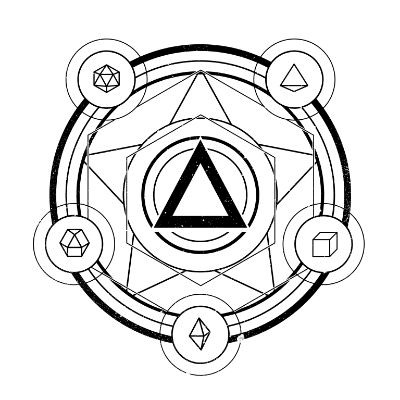
\includegraphics[width = 0.4\linewidth]{cantrip_logo.jpg}
\end{center}
\section{0-level spells}
\textit{This optional rule can be used to make the magic user ever so slightly more mischievous. Copied from \href{http://saveordie.info/?p=90}{saveordie.info}}

The Cantrip is a tiny spell created by practicing students of the magical arts during their apprenticeship and while a minor dweomer they still have some uses to the adventuring Magic-User. Elves do not obtain cantrips at first level as they don’t learn such in their youth, though a friendly Magic User may teach them at a later date.

Cantrips are cast like normal spells, only the number that a Magic User may keep in their mind at one time is equal to their Magic User level plus their Intelligence bonus. Therefore, a 1st level MU with a 16 Intelligence (+2) would start with 3 cantrips, while a 6th level MU with a 13 Intelligence (+1) would be capable of casting up to 7. As with other spells, cantrips may be memorized multiple times as desired. If a caster wished, 4 cantrips could be memorized in lieu of a 1st level spell.

A 1st level Magic User starts out with 1d4 + Intelligence modifier of cantrips known and written in their spell book. Others may be obtained during adventures just as any other spell.\\

\textbf{Spells:}
\begin{itemize}
	\item Anatomics
	\item Bug
	\item Clean
	\item Enrich
	\item Exterminate
	\item Firefinger
	\item Hairy
	\item Haunting
	\item Legerdemain
	\item Repair
	\item Temperature
	\item Transmogrify
	\item Unseen Hand
\end{itemize}

\begin{samepage}
\textbf{Anatomics (Evocation)}\\
Level: 0\\
Area of Effect: One person\\
Duration: 1 action\\
Saving Throw?: None

\nopagebreak	
When this cantrip is cast, the subject will involuntarily emit a body noise or reaction of the casters choosing. Such simple reactions can be a belch, blink, nod, yawn, etc; but nothing sophisticated
\end{samepage}

\begin{samepage}	
\textbf{Bug (Summoning)}\\
Area of Effect: 10 feet\\
Duration: Permanent\\
Saving Throw?: None

\nopagebreak
When this cantrip is used, the caster summons an insect from someplace — where is of no importance, for the creature appears in seconds. The bug will appear in whatever spot the caster is gazing at, up to a 10 foot distance from him or her. The bug is, of course, annoyed, and it is 90\% likely to sting or bite (if possible) any living creature it finds itself upon. (This will certainly cause the subject to react violently if it would otherwise be so affected by such).
\end{samepage}

\begin{samepage}	
\textbf{Clean (Abjuration)}\\
Area of Effect: 4 sq. yards\\
Duration: Permanent\\
Saving Throw?: None
	
\nopagebreak
This cantrip enables the caster to remove heavy soil, dirt, and like foreign objects from floors, walls, dishes, windows, clothing, etc. The subject surfaces are then spotless, but care must be taken in removal of pigments and the like, so usually only one type of material will be treated in a single application. The reverse of this cantrip dirties and befouls any surface equal to the area of effect.
\end{samepage}

\begin{samepage}	
\textbf{Enrich (Enchantment)}\\
Area of Effect: One object\\
Duration: Up to 6 turns\\
Saving Throw?: None

\nopagebreak
This cantrip enables the caster to give the subject a superior or better or different aspect of its to the senses; be they sight, smell, sound, touch or taste. Thus, mush can be made to taste as if it were lobster bisque, but the dweomer will not actually affect quality or wholesomeness. It can also be used to restore faded hues or to tinge those already colored with a different hue. A rough canvas garment can be made to feel like silk or velvet. A rotten egg can smell like fresh daisies, and a irritating sound can be made to sound like a canary’s song. However, the cantrip may only effect one sense per casting.
\end{samepage}

\begin{samepage}	
\textbf{Exterminate (Abjuration)}\\
Area of Effect: One small creature\\
Duration: Permanent\\
Saving Throw?: See below

\nopagebreak
When this cantrip is used, the caster may kill a small pest such as a fly, mouse, (non-giant) rat, beetle, or the like. It is useful for indoor and outdoor applications. If the subject is very small, an area of up to 1/2 cubic foot can be rid of pests. This cantrip is effective against magical creations and normal-sized creatures magically shrunk to insect-size, with a saving throw applicable to negate. The dweomer however has no effect on polymorphed creatures and similarly enchanted beings.
\end{samepage}

\begin{samepage}	
\textbf{Firefinger (Alteration)}\\
Area of Effect: 1/3' line\\
Duration: 1 round\\
Saving Throw?: None

\nopagebreak	
The firefinger cantrip enables the caster to cause a jet of flame up to one-half foot in length to shoot forth from his or her finger. The flame is very hot and will ignite combustible materials such as parchment, twigs, kindling, and the like without difficulty, providing the materials are relatively dry. The flame persists for up to 1 round.
The reverse of this Cantrip extinguishes a small flame such as used in a lantern or candle. A torch is too large a flame to be effected with this cantrip.
\end{samepage}

\begin{samepage}	
\textbf{Hairy (Alteration)}\\
Area of Effect: One object\\
Duration: Permanent\\
Saving Throw?: None

\nopagebreak	
While this cantrip is not actually one of the standard useful ones which apprentices reverse for mischievousness, it is one which is generally used for no good purpose. It causes hair, fur, or hairlike growth to thicken and lengthen. Thus, a head of hair, a peach, a beard, a cat, or whatever could be affected. The growth will cause the subject material to increase from 2-12 inches in length. The subject material must be trimmed or cut to remove the cantrip’s effect. This cantrip can be reversed to shorten growth or effectively shave, but since the effect on short material (growth under 1 inch in length) is complete absence of growth for 2-12 days, it is not often used.
\end{samepage}

\begin{samepage}	
\textbf{Haunting (Illusion)}\\
Area of Effect: Special\\
Duration: See below\\
Saving Throw?: Yes

\nopagebreak
This cantrip creates the illusion of any number of ghostly sounds such as a faint groan, creak, footfalls, etc. Naturally, those creatures within hearing distance are allowed a saving throw versus spell, and if it succeeds, the individual will hear no such noise. The sound only lasts from 1-20+ Magic User’s level in seconds.
\end{samepage}

\begin{samepage}
\textbf{Legerdemain (Illusion)}\\
Area of Effect: One small item\\
Duration: 1 round\\
Saving Throw?: None

\nopagebreak
This cantrip enables the caster to secret or cause to appear a small object in his hand without seeming to do so. The item created to appear from nowhere is illusory, and will disappear in 1 round.
\end{samepage}

\begin{samepage}	
\textbf{Repair (Alteration)}\\
Area of Effect: One object\\
Duration: Permanent\\
Saving Throw?: None

\nopagebreak	
This cantrip repairs small breaks in objects. It will weld a broken ring, chain link, medallion or ripped material, providing but one break exists. Ceramic or wooden objects with multiple breaks can be invisibly rejoined to be as strong as new. A hole in a leather sack or wineskin is completely healed over by a Repair cantrip. This cantrip will not repair magic items of any kind.
\end{samepage}

\begin{samepage}	
\textbf{Temperature (Evocation)}\\
Area of Effect: 1' cube\\
Duration: Special\\
Saving Throw?: none

\nopagebreak
A cantrip of this nature allows the caster to cause non-living liquid or solid material to become about 40°F. warmer or cooler than it was, subject to a minimum temperature of freezing. The warming or chilling effect lasts for but an instant, after which the subject returns slowly back to ambient temperature as normal for the current climate.
\end{samepage}

\begin{samepage}	
\textbf{Transmogrify (Alteration)}\\
Area of Effect: One creature/item\\
Duration: See below\\
Saving Throw?: See below

\nopagebreak
By means of a transmogrify cantrip, the caster alters one small object to another, although the change must be within the same kingdom, and only animal and vegetable objects are affected. Thus, a piece of parchment can be changed to a brightly colored cloth square, then the cloth can be changed to a rose by another use of the cantrip. Likewise, a bird can be changed into a bat, the bat to a flying squirrel by another use of the same type of cantrip, and so forth. Each alteration requires a transmogrify cantrip. The cantrip will not cause more than a 50\% increase or decrease in size/volume, and the effect will last for a base time of 1 turn. If the change is radical, then the time will be reduced accordingly; i.e., changing a dead object to a live one is a radical change and will last only 1 round. On the other hand, a very slight alteration such as color change or the like will last for 1 or more days. A saving throw against this magic does not apply as long as small, animal-intelligence, non-magical creatures of normal sort are concerned.
\end{samepage}

\begin{samepage}	
\textbf{Unseen Hand (Conjuration)}\\
Area of Effect: One creature/item\\
Duration: 1 action\\
Saving Throw?: Save vs. Magic to avoid a 1 round distraction.

\nopagebreak
By means of this cantrip, the caster causes an unseen hand to perform simple actions such as open/close a door, lift a small object and carry it (1 lb limit) within 10 feet radius of the caster, and poke or pinch a target as desired.
If this cantrip is used on a spellcaster, the target must make a saving throw vs. magic, with success meaning that the target is not distracted. Failure causes a 1 round distraction and may interrupt spell casting at DM’s discretion.\\
\end{samepage}

\vspace{0.5cm}
\part*{Cursed Artifacts}
\vspace{0.5cm}

\begin{center}
	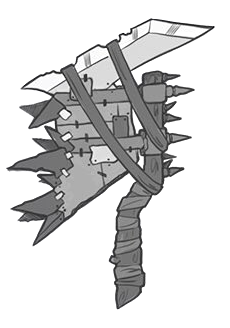
\includegraphics[width = 0.3\linewidth]{Garthruks_axe.png}
\end{center}
\section{The Axe of Garthruk}
\textit{A blackened axe made with crude green metal. It angrily shakes when approached.}

Garthruk the Orc Chief is captured within the axe. He wants to challenge the great and mighty, and escape his metal prison.

Abilities:
\begin{itemize}
	\item \textbf{Orcish Strength:} The wielder's muscles bulge and he suddenly can perform orcish feats of strength.
	\item \textbf{Possession:} When triggered, Garthruk will try to possess the wielder. Save against Paralysis or be possessed for 3d6 minutes by a raging Orc. Possession occurs when one of the following conditions is met:
	\begin{itemize}
		\item Attempting to get rid of the axe (automatic possession, no save allowed).
		\item Evading a mighty foe.
		\item Failing to protect your honor.
	\end{itemize}
	\item \textbf{Corruption:} Every failed save gives the wielder an Orc point. After the wielder reached his Orc threshold - 2d6 rolled in secret by the GM after touching the axe - the wielder will count as being an Orc instead of his/her former race.
\end{itemize}
Stages: 
\begin{itemize}
	\item \textbf{Stage 1 (1 Orc point}:) The wielder's face becomes cruder ever so slightly. His/her speech becomes rougher. 
	\item \textbf{Stage 2 (Orc threshold/2, rounded down):} The wielder becomes a half-Orc.
	\item \textbf{Stage 3: (Orc threshold):} The wielder is now a full-fledged Orc.
\end{itemize}

\end{document}
